% !TeX root = RJwrapper.tex
\title{Current status and propsects of R-packages for the design of
experiments}
\author{by Emi Tanaka}

\maketitle

\abstract{%
An abstract of less than 150 words.
}

\begin{Schunk}
\begin{table}

\caption{\label{tab:bigram-title}The bigram of the R-package titles as provided in the DESCRIPTION file in CRAN.}
\centering
\begin{tabular}[t]{l|r}
\hline
Bigram & Count\\
\hline
optimal design & 10\\
\hline
experimental design & 8\\
\hline
clinical trial & 5\\
\hline
dose finding & 5\\
\hline
sequential design & 5\\
\hline
block design & 4\\
\hline
microarray experiment & 4\\
\hline
response surface & 4\\
\hline
\end{tabular}
\end{table}

\end{Schunk}

\begin{Schunk}
\begin{table}

\caption{\label{tab:bigram-desc}The bigram of the R-package descriptions as provided in the DESCRIPTION file in CRAN.}
\centering
\begin{tabular}[t]{lr}
\toprule
Bigram & Count\\
\midrule
experimental design & 11\\
optimal design & 10\\
package provide & 7\\
response surface & 7\\
factorial design & 6\\
\addlinespace
graphical user & 6\\
user interface & 6\\
block design & 5\\
contour plot & 5\\
design based & 5\\
\addlinespace
effect model & 5\\
fractional factorial & 5\\
microarray experiment & 5\\
mixed effect & 5\\
provide function & 5\\
\addlinespace
sample size & 5\\
sequential design & 5\\
\bottomrule
\end{tabular}
\end{table}

\end{Schunk}

\begin{Schunk}
\begin{Soutput}
#> `stat_bin()` using `bins = 30`. Pick better value with `binwidth`.
\end{Soutput}


\begin{center}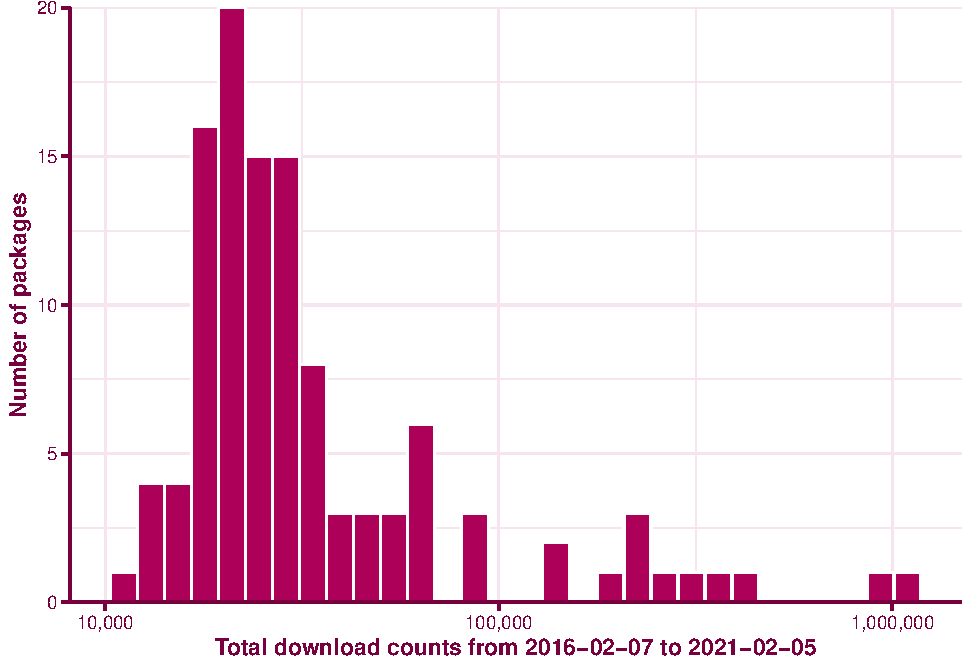
\includegraphics{paper_files/figure-latex/download-hist-1} \end{center}

\end{Schunk}

\begin{Schunk}


\begin{center}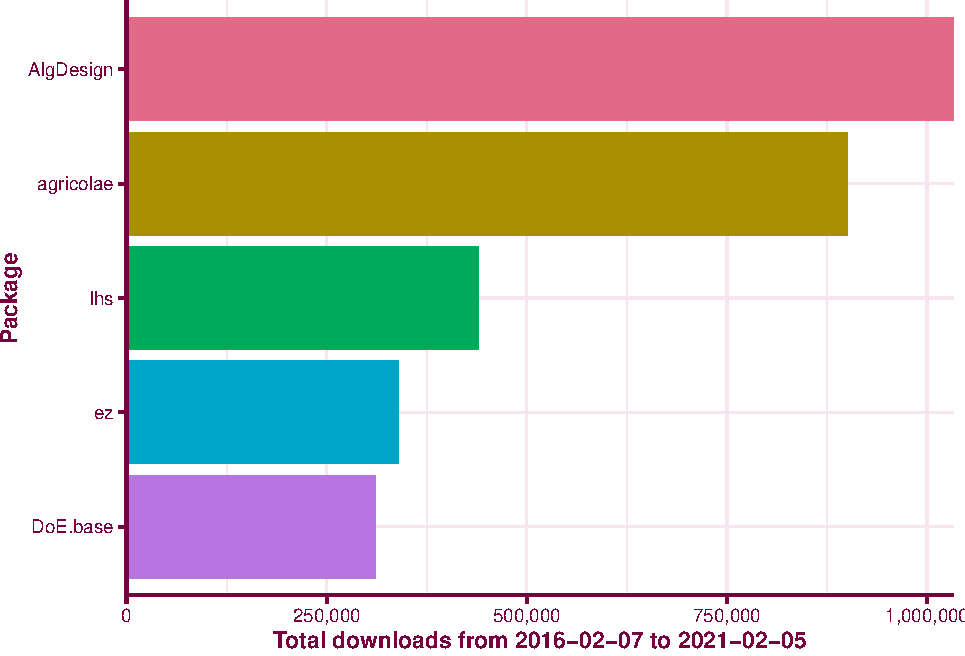
\includegraphics{paper_files/figure-latex/download-barplot-1} \end{center}

\end{Schunk}

\begin{Schunk}


\begin{center}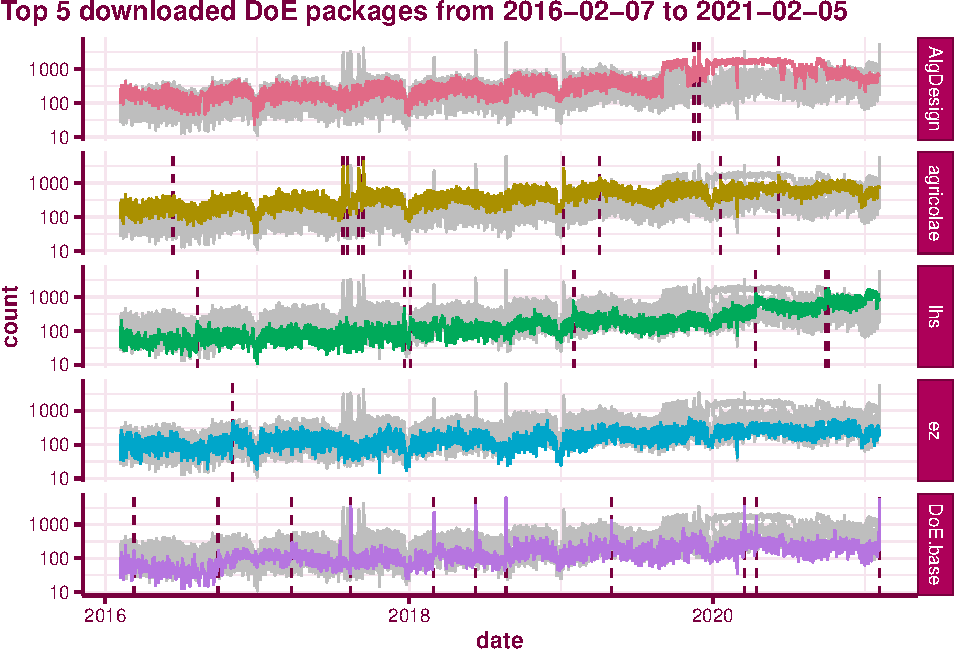
\includegraphics{paper_files/figure-latex/download-timeplot-1} \end{center}

\end{Schunk}

\hypertarget{introduction}{%
\subsection{Introduction}\label{introduction}}

\texttt{test} \code{test}

\CRANpkg{agricolae}

\ctv{ExperimentalDesign}

\ctv{OfficialStatistics}

\hypertarget{helping-info-to-get-started}{%
\subsection{Helping info to get
started}\label{helping-info-to-get-started}}

Introductory section which may include references in parentheses
\citep{R}, or cite a reference such as \citet{R} in the text.

\hypertarget{section-title-in-sentence-case}{%
\subsection{Section title in sentence
case}\label{section-title-in-sentence-case}}

Let's check fi this works Figure @ref(fig:Rlogo).

This section may contain a figure such as Figure \ref{fig:Rlogo}.

\begin{Schunk}
\begin{figure}[htbp]

{\centering 
\includegraphics[width=2in]{/Users/etan0038/Dropbox/projects/paper-review-DoE-pkgs/Rlogo} 

}

\caption[The logo of R]{The logo of R.}\label{fig:Rlogo}
\end{figure}
\end{Schunk}

\hypertarget{summary}{%
\subsection{Summary}\label{summary}}

This file is only a basic article template. For full details of
\emph{The R Journal} style and information on how to prepare your
article for submission, see the
\href{https://journal.r-project.org/share/author-guide.pdf}{Instructions
for Authors}.

\hypertarget{about-this-format-and-the-r-journal-requirements}{%
\subsubsection{About this format and the R Journal
requirements}\label{about-this-format-and-the-r-journal-requirements}}

\texttt{rticles::rjournal\_article} will help you build the correct
files requirements:

\begin{itemize}
\tightlist
\item
  A R file will be generated automatically using \texttt{knitr::purl} -
  see \url{https://bookdown.org/yihui/rmarkdown-cookbook/purl.html} for
  more information.
\item
  A tex file will be generated from this Rmd file and correctly included
  in \texttt{RJwapper.tex} as expected to build \texttt{RJwrapper.pdf}.
\item
  All figure files will be kept in the default rmarkdown
  \texttt{*\_files} folder. This happens because
  \texttt{keep\_tex\ =\ TRUE} by default in
  \texttt{rticles::rjournal\_article}
\item
  Only the bib filename is to modifed. An example bib file is included
  in the template (\texttt{RJreferences.bib}) and you will have to name
  your bib file as the tex, R, and pdf files.
\end{itemize}

\bibliography{paper.bib}

\address{%
Emi Tanaka\\
Monash University\\%
Monash University\\ Clayton campus, VIC 3800, Australia\\
%
\url{http://emitanaka.org/}%
\\\textit{ORCiD: \href{https://orcid.org/0000-0002-1455-259X}{0000-0002-1455-259X}}%
\\\href{mailto:emi.tanaka@monash.edu}{\nolinkurl{emi.tanaka@monash.edu}}
}
